\documentclass[crop,tikz,dvipsnames]{standalone}
\usepackage{xcolor}
\usepackage{amsfonts}
\usepackage{amsthm}
\usepackage{amsmath}
\usetikzlibrary{positioning}
\begin{document}
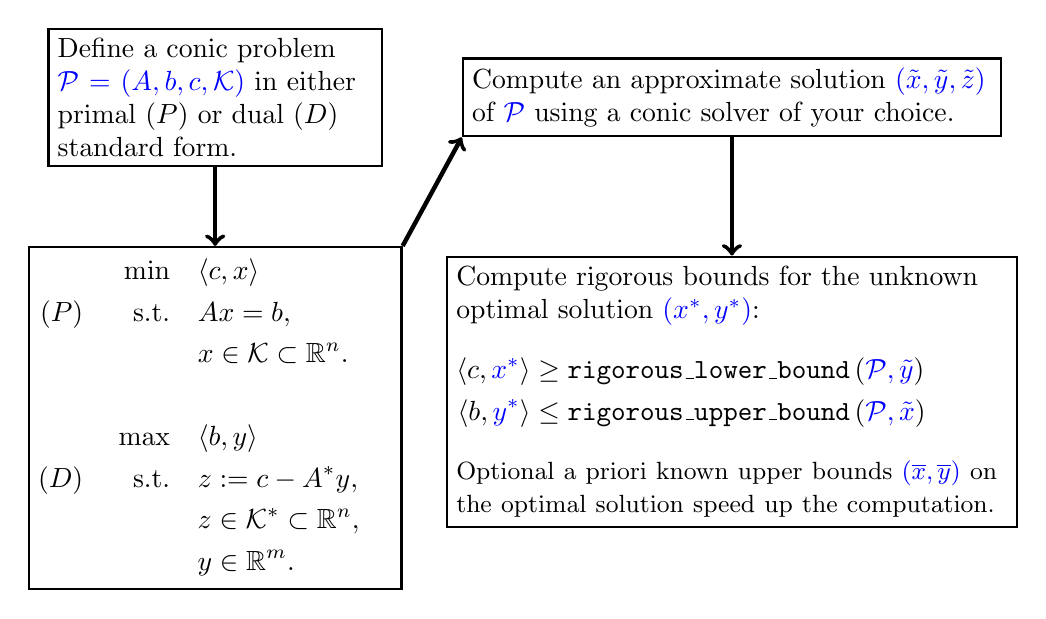
\begin{tikzpicture}
\node[text width=4cm,draw,thick] (step1) {
Define a conic problem
{\color{blue} $\mathcal{P} = (A,b,c,\mathcal{K})$}
in either primal $(P)$ or dual $(D)$ standard form.
};
\node[below =of step1,text width=4.5cm,draw,thick] (step2) {
$\begin{aligned}
    &\;&        \min &\quad \langle c, x \rangle \\
(P) &\;& \text{s.t.} &\quad Ax = b, \\
    &\;&             &\quad x \in \mathcal{K} \subset \mathbb{R}^{n}.\\
\\
    &\;&        \max &\quad \langle b, y \rangle \\
(D) &\;& \text{s.t.} &\quad z:= c - A^{*}y, \\
    &\;&             &\quad z \in \mathcal{K}^{*} \subset \mathbb{R}^{n},\\
    &\;&             &\quad y \in \mathbb{R}^{m}.
\end{aligned}$
};
\node[right =of step1,text width=6.6cm,draw,thick] (step3) {
Compute an approximate solution
{\color{blue} $(\tilde{x},\tilde{y},\tilde{z})$}
of {\color{blue} $\mathcal{P}$} using a conic solver of your choice.
};
\node[below =1.5cm of step3,text width=7.0cm,draw,thick] (step4) {
Compute rigorous bounds for the unknown optimal solution
{\color{blue} $(x^{*},y^{*})$}:
\\[1em]
$\begin{aligned}
\langle c, {\color{blue} x^{*}} \rangle &
\geq \texttt{rigorous\_lower\_bound}\,({\color{blue} \mathcal{P}, \tilde{y}}) \\
\langle b, {\color{blue} y^{*}} \rangle &
\leq \texttt{rigorous\_upper\_bound}\,({\color{blue} \mathcal{P}, \tilde{x}})
\end{aligned}$
\\[1em]
{\small
Optional a priori known upper bounds
{\color{blue} $(\overline{x},\overline{y})$}
on the optimal solution speed up the computation.}
};
\draw[->,ultra thick] (step1.south) -- (step2.north);
\draw[->,ultra thick] (step2.north east) -- (step3.south west);
\draw[->,ultra thick] (step3.south) -- (step4.north);
\end{tikzpicture}
\end{document}
